\chapter{Interprocess Communication}
\textbf{Communication between processes is essential to allow them to cooperate and reach specific goals.} Interprocess communication defines how processes communicate inside the network.
\begin{itemize}
    \item \textbf{Remote Procedure Call:} allowing a calling process to call a procedure in a remote node as if it is local
    \item \textbf{Remote Method Invocation:} remote objects are called with a remote invocation. It is necessary to maintain a remote interface to give information about what kind of methods the object offers and how remote processes can invoke them
    \item \textbf{Events:} asynchronous notification to objects of events
\end{itemize}

\section{Transparency and Implementation}
One aspect that is very important for an IPC is the \textbf{level of transparency provided to the processes.} The main goal is to \textbf{call remote procedures as they are local}. In this case \textbf{RPC} offers the \textbf{maximum level of transparency}, but it has some \textbf{problems distinguishing local and remote procedures}. The development of RPC and RMI includes:
\begin{itemize}
    \item \textbf{Marshalling:} technique to codify parameters in order to be sure that the structure given to the procedure is preserved. This problem arises from the possibility of a computer system to represent data in different ways. Marshalling codifies parameters to transform them into a common representation, improving reliability and performance
    \item \textbf{Invocation semantic:}  determines what kind of semantic is given to the processes
    \item \textbf{Binding:} strategy to \textbf{identify and connect to the server}
        \begin{itemize}
            \item \textit{Static:} decided a priori how to reach the server -> faster since there is a direct communication to the server
            \item \textit{Dynamic:} discovers where is the server dynamically \(\rightarrow\) higher level of \textbf{location transparency}
        \end{itemize}
\end{itemize}
The \textbf{Middleware} provides \textit{transparency}, the procedure calls are used in the same way if they are local or remote. It supports implementation for RPC and RMI and if the middleware allows different programming languages, it usually specifies the final notation using an \textbf{Interface Definition Language (IDL)}.
\textbf{Interfaces} are implemented in order to \textbf{make the operations transparent}, programs are organized in a set of modules that cooperate. The interface has \textbf{only the information needed for available methods and it doesn’t define the final implementation.}

\section{Object Oriented Model}
RMI is based on the \textbf{Object Oriented Model (OOM)}, in which components are called objects. An \textbf{object} is an entity that contains a set of data and methods that define its behavior.
OOM offers:
\begin{itemize}
    \item \textbf{Reference to object:} it is an alternative \textit{identifier for an object}. Objects can be passed as arguments or obtained as results
    \item \textbf{Interface:} it defines \textit{methods} and how to use them but it does not specify how they are implemented.
    \item \textbf{Methods:} are operations that define the \textit{behavior of objects of the same class}
\end{itemize}
Usually Object Oriented Programming languages are supported by an entity called \textbf{Garbage Collector}, used to recover memory space of objects that are not referenced.

Example of interaction using remote and local methods:
\begin{enumerate}
    \item Object A invokes a remote invocation to object B, since it is out of the environment of A.
    \item Later B invokes local methods of C and D
    \item At the end E applies a remote invocation to a method of F, since they are inside the same system but in different environments
    
    \begin{figure}[!h]
            \centering
            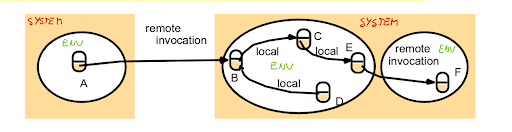
\includegraphics[width=.7\linewidth]{images/InterprocessCommunication/exampleOOP.png}
            \caption{Example of usage of remote and local methods}
    \end{figure}
    
\end{enumerate}

\section{Invocation Semantics}
Remote procedure calls provide a range of invocation semantics that specify the implementation of the \textbf{invocation of the protocol Request-Reply}. Invocation semantics are defined in base of different implementation choices considering:
\begin{itemize}
    \item Re-transmission of the request
    \item Duplicate filtering in the server in the case of re-transmission
    \item At arrival of a re-transmitted request: re-execution of resend of the result 
\end{itemize}
There can be \textbf{different types of call semantics}, referring to the reliability of the RPC or RMI from the caller point of view. Local operations guarantee Exactly Once semantic, since the caller knows that the request will be sent and executed exactly once.

\begin{figure}[!h]
            \centering
            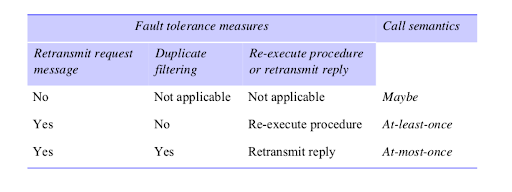
\includegraphics[width=.7\linewidth]{images/InterprocessCommunication/invocationSemantcs.png}
            \caption{Invocation Semantics}
    \end{figure}

\begin{itemize}
    \item \textbf{Maybe:} the request is \textbf{sent only once} independently of the fact that the client receives a reply or not
        \begin{itemize}
            \item There is \textbf{no fault tolerance measure}, there might be loss of the invocation or the result or crashing of the server.
            \item The client does not know if the RMI or RPC has been \textbf{successful or not.}
        \end{itemize}
    \item \textbf{At least once:} there is \textbf{re-transmission until the client does not get a reply}.
        \begin{itemize}
            \item Possible duplicate executions
            \item It can be used only for \textbf{idempotent operations} \(\rightarrow\) operations that return the same result at every execution and that do not produce any change of state.
        \end{itemize}
    \item \textbf{At most moce:} there is \textbf{re-transmission until the client does not get a reply}, but the server \textbf{remembers the operations already executed} and does not reply to the same operations.
        \begin{itemize}
            \item The server maintains an \textbf{history table} in which stores client id and operations executed for him
            \item When a \textbf{request arrives} to the server it verifies if the request has \textbf{already been performed} for the same client
                \begin{itemize}
                    \item \textit{Positive answer:} it returns the result without replay the execution
                    \item \textit{Negative answer:} it compute and return the result
                \end{itemize}
        \end{itemize}
    \item Operations for this semantic are called \textbf{non-idempotent}, since each time they are executed, they produce a change of state inside the server
\end{itemize}

RPC and RMI are very similar, the choice of adopting one of them essentially regards the programming language adopted, for instance oop languages (like Java) tend to adopt RMI

\section{RMI}
\begin{itemize}
    \item \textbf{Communication module:} it is responsible for \textbf{providing a specified invocation semantic.} There are 2 communication modules, one inside the \textbf{client environment} and the other one inside the \textbf{server environment}. The two components carry out the request-reply protocol between client and server
    \item \textbf{Remote reference module:} it is responsible for the \textbf{translation between local and remote object references and for creating remote object references.} It contains a remote object table that records the correspondence between local object references in that process and remote object references
    \item \textbf{Proxy:} it makes remote method invocation transparent to the client, it is also responsible for marshalling and un-marshalling
    \item \textbf{Dispatcher:} it is defined inside the server. When it receives a request message from the communication module, it \textbf{selects the appropriate method in the skeleton required by the request}
    \item \textbf{Skeleton:} it implements the methods in the remote interface
    
    \begin{figure}[!htb]
       \begin{minipage}{0.48\textwidth}
         \centering
         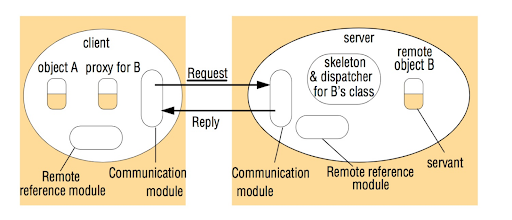
\includegraphics[width=.99\linewidth]{images/InterprocessCommunication/rmi1.png}
       \end{minipage}\hfill
       \begin{minipage}{0.48\textwidth} 
         \centering
         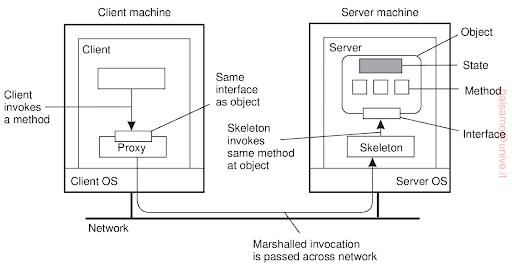
\includegraphics[width=.99\linewidth]{images/InterprocessCommunication/rmi2.png}
       \end{minipage}
    \end{figure}
        
\end{itemize}

\section{RPC}
\begin{itemize}
    \item \textbf{Stub:} its main role is to make \textbf{transparent the remote call} and \textbf{execute marshalling}
        \begin{itemize}
            \item \textit{Client stub} makes transparent the remote call and execute marshalling
            \item \textit{Server stub} applies un-marshalling and execute the service procedure required
        \end{itemize}
    \item \textbf{Dispatcher:} it opens the request message and it selects the procedure corresponding to the request
    
    \begin{figure}[!h]
            \centering
            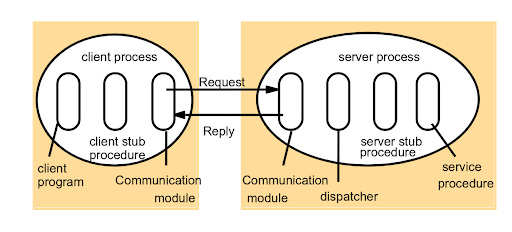
\includegraphics[width=.7\linewidth]{images/InterprocessCommunication/rpc.png}
            \caption{RPC}
    \end{figure}
    
\end{itemize}

\newpage

\section{Callback}
In some cases a client can send continuous requests to the server and in this way the transmission delay and waiting time have a strong effect on the performance.
Request-Reply protocol is not ideal so a possible solution is to reverse the interaction:
\begin{itemize}
    \item Server notifies the client when it is available
    \item The client sends a remote object containing a methods that the server can invoke
    \item The server keeps a list of records containing clients and their requests
\end{itemize}
When an \textbf{event} occurs the server calls all the interested clients

\textbf{Advantages:} it avoids repeated calls from the clients that increase the performances

\textbf{Disadvantages:} the server has to keep a list of the interested clients and realize RMI to all the callback in the list

\begin{figure}[!h]
            \centering
            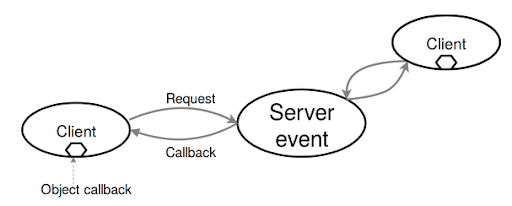
\includegraphics[width=.7\linewidth]{images/InterprocessCommunication/callback.png}
            \caption{Callback}
    \end{figure}
